\documentclass[11pt,titlepage,openright]{book}
\usepackage[utf8]{inputenc}
\usepackage[T1]{fontenc}
\usepackage[british]{babel}
\usepackage{graphicx}
\usepackage[dvipsnames]{xcolor}
\usepackage{libertine}
\renewcommand*\ttdefault{cmtt}

\usepackage[sf]{titlesec}
\usepackage[square]{natbib}
\setcitestyle{numbers} 
%\usepackage[export]{adjustbox}

\usepackage{
  paralist,   % Improved lists 
  marginnote, % Improved margin notes
  environ,
  ragged2e,   % Justified text in the margin notes
  url,        % For typesetting URLs
  listings,   % Code formatting
  hyperref,   % Links in PDF from TOC, refs, etc.
  lipsum,
  wrapfig     % For wrapping figures in text
}
\lstset{
  inputpath=scripts/,
  breaklines=true
  }
\usepackage{changepage}
\usepackage{float}
\usepackage[list=true,]{subcaption}

\usepackage[twoside,labelfont=sf]{caption}

\graphicspath{{images/}{images/graphs/}}

\captionsetup{justification=raggedright,singlelinecheck=false}

\newcommand\myhrulefill[1]{\leavevmode\leaders\hrule height#1\hfill\kern0pt}
\DeclareCaptionFormat{FigFormat}{{\color{black}\myhrulefill{0.5pt}}\\#1#2#3}
%\captionsetup[figure]{format=FigFormat}
%\captionsetup[table]{format=FigFormat}

\DeclareCaptionFormat{LstFormat}{\textsf{Listing}~\arabic{chapter}.\arabic{listing}:#2#3}
\floatstyle{ruled}
\newfloat{listing}{thp}{lol}
\floatname{listing}{Listing}
%\captionsetup[listing]{format=LstFormat}


\NewEnviron{MarginNote}[1][0mm]{\marginnote{\footnotesize\justifying\BODY}[#1]}
\newcommand{\Footnote}[2][0mm]{\footnotemark\marginnote{\footnotesize$^{\arabic{footnote})}$~#2}[#1]}

\renewenvironment{figure*}[1][]{%
  \begin{figure}[#1]%
    \checkoddpage%
    \ifoddpage%
      \begin{adjustwidth}{0cm}{-45mm}%%
    \else%
      \begin{adjustwidth}{-45mm}{0cm}%%
    \fi%
    }{%
    \end{adjustwidth}%
  \end{figure}}

\renewenvironment{table*}[1][]{%
  \begin{table}[#1]%
    \checkoddpage%
    \ifoddpage%
      \begin{adjustwidth}{0cm}{-45mm}%%
    \else%
      \begin{adjustwidth}{-45mm}{0cm}%%
    \fi%
    }{%
    \end{adjustwidth}%
  \end{table}}

\renewenvironment{listing*}[1][]{%
  \begin{listing}[#1]%
    \checkoddpage%
    \ifoddpage%
      \begin{adjustwidth}{0cm}{-45mm}%%
    \else%
      \begin{adjustwidth}{-45mm}{0cm}%%
    \fi%
    }{%
    \end{adjustwidth}%
  \end{listing}}

%% == Code =======================================================
\lstnewenvironment{Code}[1][style=std]{\lstset{#1}}{}
\lstnewenvironment{Code_Numbered}[1][style=std,numbers=left]{\lstset{#1}}{}

\renewcommand{\c}[1]{\lstinline[style=std]@#1@}

\lstdefinestyle{std}{
  language=python,
  basicstyle=\small\sf\color{black},
  keywordstyle=\small\sf\bfseries,
  numberstyle=\footnotesize\sf\color{black},
  commentstyle=\small\color{black}\it,
  aboveskip=1ex,
  belowskip=1ex,
  tabsize=2,
  columns=fullflexible,
  xleftmargin=1ex,
  resetmargins=true,
  showstringspaces=false,
  morecomment=[l]{//},
  morecomment=[l]{--},
  morecomment=[s]{/*}{*/},
  escapeinside=@@,
  morekeywords={Frobies},
  moredelim=[is][\textit]{___}{___},
  moredelim=[is][\textbf]{__*}{*__}
}

\usepackage[activate={true,nocompatibility},final,tracking=true,kerning=true,spacing=false,factor=1100,stretch=10,shrink=10]{microtype}
\usepackage[paper=a4paper,text={13cm,24cm},marginparsep=5mm,marginparwidth=45mm,inner=20mm,twoside]{geometry}

\newcommand{\RED}[1]{\textcolor{red}{#1}}
\newcommand{\ie}{\emph{i.e.,}}
\newcommand{\eg}{\emph{e.g.,}}
\newcommand{\etal}{\emph{et~al.}}

\renewcommand{\bfdefault}{b}
\clearpage{\pagestyle{empty}\cleardoublepage}

\synctex=1
\pagestyle{plain}

\begin{document}
\frontmatter
\title{Implementing NB-IoT: Communication with a Load Cell}
\author{Johannes Almroth}
\date{\today}

\maketitle

\vspace*{3cm}
\section*{Acknowledgements}
Many thanks to Vetek, who funded the purchase of all the hardware equipment used in the project.

Many thanks to the Communication Research Lab at Uppsala university for providing me with space and tools to conduct my work.

Many thanks to Laura Feeney PhD, for your outstanding patience, words of encouragement as well as your time. 

Many thanks to professor Per Gunningberg for reviewing my paper

Many thanks to my partner, Sabina Smedsrud, for always cheering me up and supporting me.
\newpage

\vspace*{3cm}
\section*{Abstract}
The purpose of this project is to establish a line of communication between a loading cell and the internet. This will be done through the NB-IoT technology, and the data being sent is the one being produced by the loading cell. Using a development board from PyCom and a SIM-card from Telia as the network service provider, [...]


\tableofcontents
\listoffigures
% \listoftables

\mainmatter

\chapter{Introduction}
% Should be 25% of the total paper

Vetek is a Swedish scale supplier located in Väddö, situated approx. 100 kilometers north of Stockholm. Vetek constructs their own scales and weighing systems, as well as reselling products from other manufacturers.\cite{vetek} 

Vetek aims to improve their services, and as such are interested in the possible use cases of IoT (Internet of Things) technology, and ultimately see how that can be applied to their own products. In this paper,the term IoT will simply mean ``(a) device(s) connected to the internet''\cite{what_is_iot}. In a pilot project, Vetek wants to see how this connectivity can be implemented in a energy-efficient and effective manner. This would entail investigating factors such as power consumption, range and data rate. NB-IoT (Narrowband-IoT), a new and emerging radio technology, encapsulates some principles suitable for this type of endeavor, such as wide coverage, low power consumption and low complexity.\cite{NB-overview} Using some form of NB-IoT compatible microcontroller and hooking it up to a basic load cell should provide sufficient testing grounds to see how this new functionality could improve existing products.


\section{Purpose and Goals}
\iffalse
\begin{itemize}
	\item Write about the grand scheme of things
	\item Set the correct expectations
	\item What can I expect to learn if I keep on reading?
	\item What are the success criteria for this work?
	\item How will the work be evaluated?
\end{itemize}
\fi

NB-IoT is a relatively new technology, and as such, implementations and documentations remain sparse. With this in mind, even a small project such as this will serve as a guiding post for future work. The goal of this project is to establish a working internet connection with a load cell through the NB-IoT technology. The data sent from the load cell should be functionally identical to the data produced if the load cell was offline. Disregarding problems due to a internet service provider, data speeds and losses should not be abnormal. Using the same components, replication of the project should be feasible with the documentation provided in this thesis, assuming software and service providers remain.

The end-goal can be divided into two sub-goals. 
\begin{itemize}
	\item Enable internet communication from the microcontroller.
	\item Enable data transfer from the load cell to the microcontroller.
\end{itemize}


\section{Delimitations}
\iffalse
\begin{itemize}
	\item Scale down expectations and clarify
\end{itemize}
\fi
The final implementation will not be a functional product ready to be used. Any extra improvements upon a internet-enabled load cell will only be done if time remains after the implementation and the completion of the thesis.

\chapter{Background}
% Should be ~2 pages 

% **Problems**

% - Too much mixed information
% - The expensive stuff is not expensive
% - Requirements should be its own chapter

% **Needs to contain**

% - More subheadings

% **Structure**

% - General Background
% - LTE-M vs NB-IoT
% - Market in Sweden

\section{General Background}
IoT has been lauded as a world-changing technology that will significantly affect our economy as well as our way of living. In a report by the GSMA, the total number of IoT devices is estimated to triple by 2025, bringing it to \$25.2 \textit{billion}.\cite{gsma-report} Meanwhile, the global IoT revenue will fourfold from 2018, increasing it to \$4.4 \textit{billion}.\cite{gsma-report} While there undeniably is a lot of excitement and potential economic impact associated with IoT, currently, many consumers just associate the term with connecting a common toaster or coffee machine to a Wi-Fi network. While this technically fits the definition for an IoT device,\cite{what_is_iot} the significant use cases will probably be implemented with different sensors, such as scales, thermometers, etc. that will further improve automatization and optimization processes. As an example, the key categories within the predicted growth are smart homes (\eg~ security devices) and smart buildings (\eg~ energy consumption sensors).\cite{gsma-report} For the predicted growth to happen, businesses need to take a chance and work on projects that implement different IoT technologies, and to enable this, the 3GPP has developed some Low-Power Wide-Area Network (LPWAN) protocols that focus on different key aspects that make IoT possible. Some of these aspect include long battery life, high connection density, indoor coverage and geo-tracking capabilities. Aside from security, one of the biggest challenges regarding IoT devices relate to limitations arising from energy infrastructure. As mentioned earlier, one of the core issues NB-IoT aims to achieve is to be a low-power technology, thus decreasing the maintenance needed for battery-powered devices. A claim often paraded with NB-IoT is that it enables a battery-time of up to 10-years,\cite{gsma-nb-iot} though it is worth mentioning that over such a period of time the underlying IoT technology (in the form of microcontrollers/sensors) will probably require more frequent maintenance than the batteries themselves.

% Background about making your own IoT sensor
% TODO: Find one articles relating to this

% Background about energy efficiency
% TODO: Find two articles relating to this

% \section{NB-IoT vs. LTE-M}
% The two most prominent of the protocols developed by the 3GPP are NB-IoT and LTE-M. To utilize the technologies, a NB-IoT or LTE-M SIM-card has to be acquired from a local network provider, and inserted into a compatible piece of software within range from a base station.

% Long-Term Evolution Machine Type Communication (LTE-M) has the most functionality, including voice capabilities and device positioning. Thanks to its wider bandwidth frequency it also has lower latency and boasts a data rate up to 1 Mbps.\cite{ericsson-blog} In return, device complexity and costs are higher compared to NB-IoT. The focus of NB-IoT was to enable indoor coverage, low cost development, long battery life and high connection density, which makes the technology ideally suited for low data rate applications in extremely challenging radio conditions. 

% \section{NB-IoT Market in Sweden}
% According to Swedish telecom company Telia, they were the first to introduce the NB-IoT technology in Sweden, as well as the Nordic countries overall.\cite{telia-nb} They further claim that their network will be in range for over 99.9\% of Sweden's population, as well as provide a speed of 200 kb/s in more than 95\% of the country.\cite{telia-first} The grand opening of the network was on the 24th of May 2019, and pilot projects were conducted as early as a year before this in multiple locations across the country. Telia currently offers a starter kit  for any actor interested in the technology, with a trial period of 6 months that includes access to Telia's IoT portal and APIs as well as 5 SIM cards, each with a 30MB data capacity per month. Telia does not seem have many strong competitors when it comes to the Swedish IoT market, though Tele2 have partnered up with Nokia to offer similar services, and according to a press release from 2018, they have rolled out both LTE-M and NB-IoT across their networks.\cite{tele2-nokia} Telenor has launched a IoT network in Norway with NB-IoT functionality in 2018\cite{telenor-iot}, and according to an exchange with their customer support, followed suite in Sweden in the beginning of October. The fact that Telia already has partnered up with a multitude of cities and companies give the indication that they have a head start in the market.

\chapter{Requirements}
% **Problems**

% - Contains a bit of background info about NB-IoT which should not be there
% - Mixes sensor readings w/ data transmissions a bit

% **Needs to contain**

% - Motivations for why we need certain requirements
% - Maybe some behavior graphs for clarification
% - What issues can arise and what we want to do about it.

% **Structure**

% - Summary of subsections at the top
% - Data transmission
% - Sensor readings
% - Sensor failure
% - Sensor disconnect

In this section we will discuss some the software requirements imposed on the IoT-enabled scale device that will be implemented, and what behavior we wish to see from the device in the case of different scenarios. These areas were chosen because of their relative simple nature, as well as their relevance to other similar devices. The purpose of these requirements is to emulate the constraints placed on devices in the real world, specifically an all-purpose IoT-scale that Vetek could use in a pilot project for evaluation and future iterations. 

There are no specific requirements set for the hardware implementation. Any additional requirements in terms of energy consumption, sizing, etc. would be too vast for the scope of this paper. 

\section{Data Polling Rate}
In most IoT devices the relevant data is provided by some form of sensor, whether it be a scale, thermometer or something entirely different.\cite{what_is_iot} The type of sensor being used has a huge impact on the IoT device, especially when considering that they have to be powered by the same energy source. The simplest way of deciding when to poll data from a sensor is to let it do so at a fixed and constant rate, often enough to be relevant, and seldom enough as to not waste precious energy. However, if within the context of the application we can conclude that no data needs to be polled (for a while), then subsequently no data will need to be sent, and thus we save energy on both ends of the system. For some applications there might even be longer periods of downtime where it is not relevant to conduct monitoring on the given sensor, \eg during nighttime, closing hours, etc. Another interesting angle is modifying the polling rate depending on the data itself. A simple example of a behavior would be to have a slower polling rate at stable values, and increase it when experiencing large enough changes. Given the conditions of an IoT device powered by batteries, it is not unreasonable to assume that readings might not always be accurate at times. Depending on the sensor, spikes and drops of false values might occur, and not taking these scenarios into account would be prudent. 

In this paper, we want the device to change its polling rate depending on the data values, such that the rate increases at periods of activity and change, and lower the rate when the data stabilizes around a given value. The device should also try to take false data values into account.

\begin{figure}[H]
\centering
	\begin{subfigure}[b]{0.3\textwidth}
    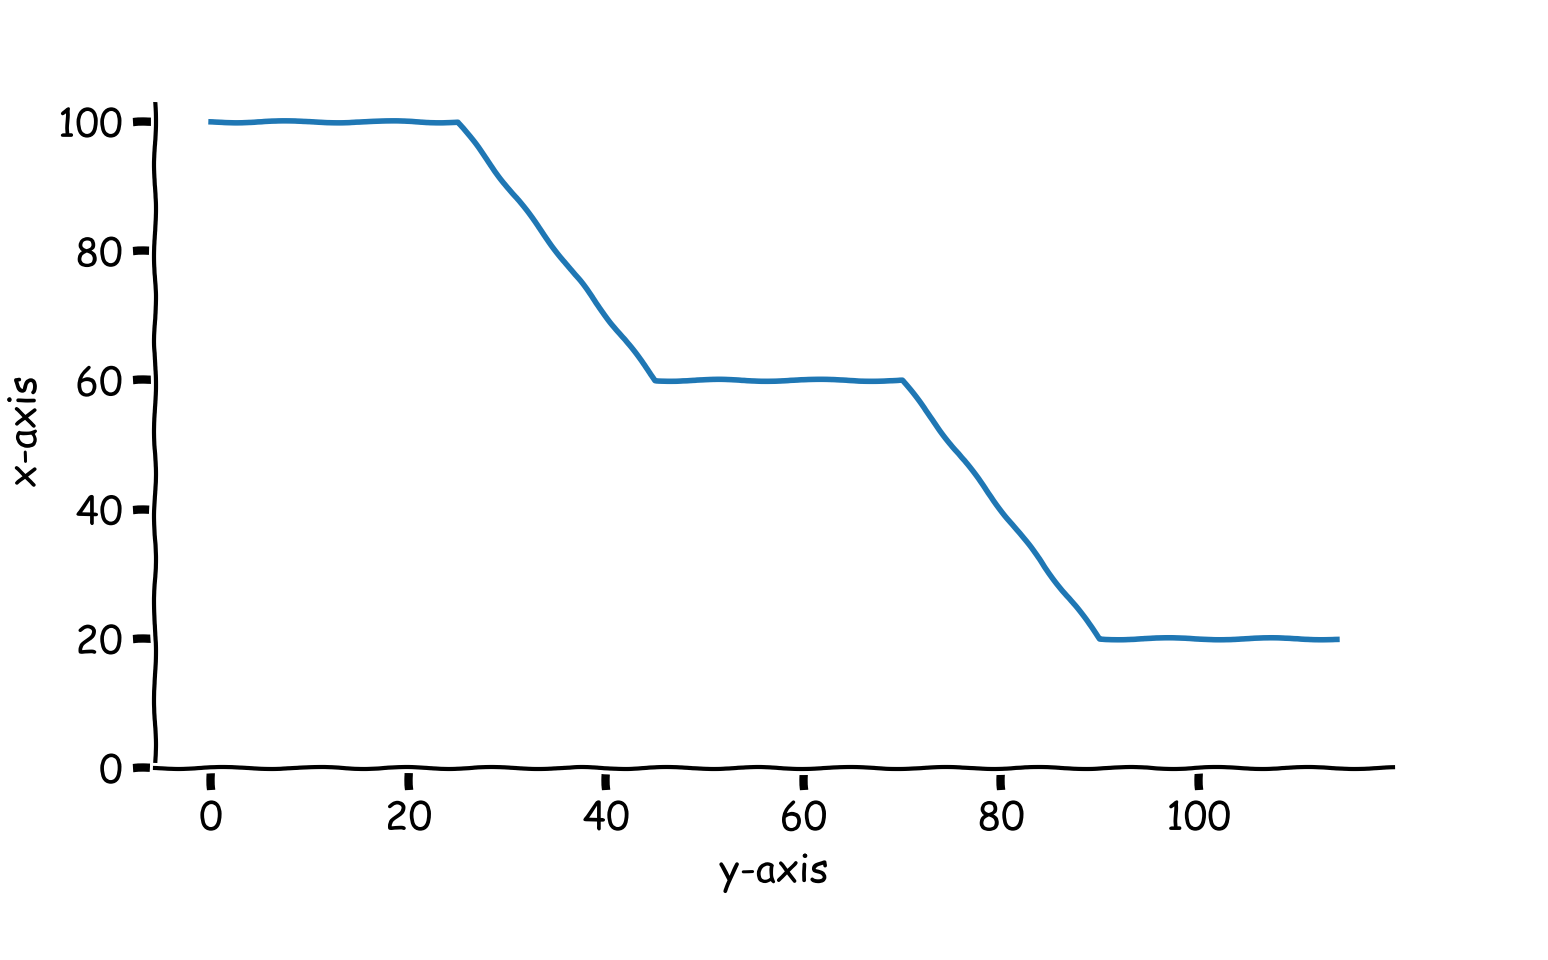
\includegraphics[width=\textwidth]{plateu.png}
    \caption{}
    \label{fig:plateu}
	\end{subfigure}
	%
	\begin{subfigure}[b]{0.3\textwidth}
    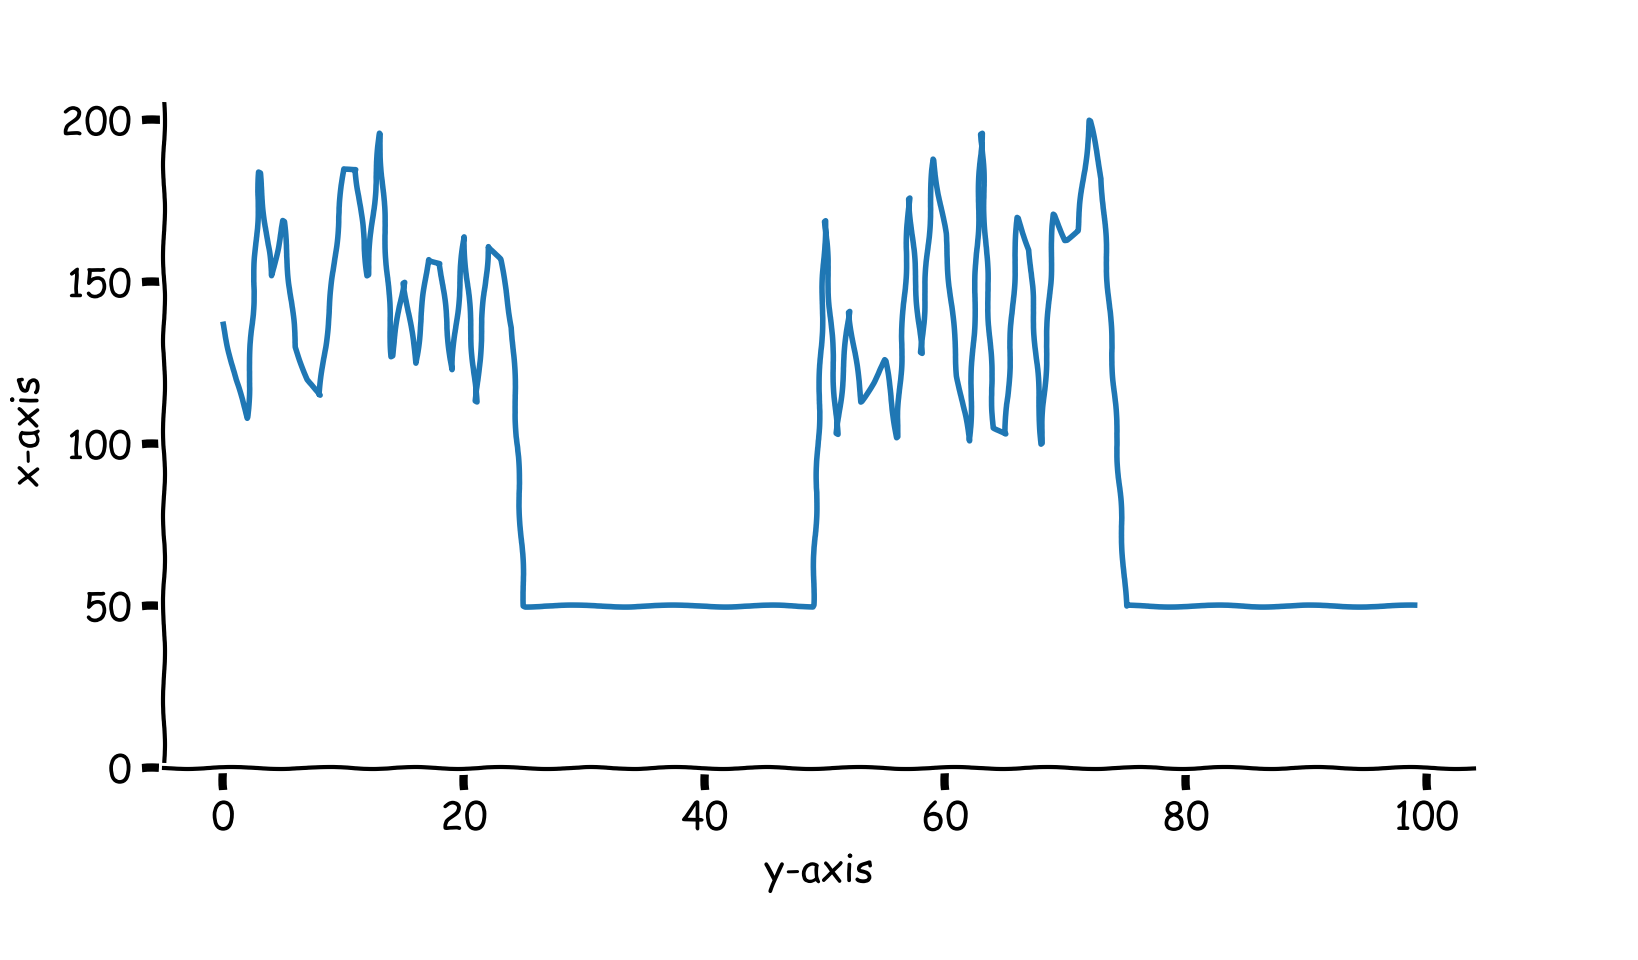
\includegraphics[width=\textwidth]{some_spikes.png}
    \caption{}
    \label{fig:spikes}
	\end{subfigure}
\caption{Graph a) shows plateauing development of values, while graph b) displays spikes in the readings}
\end{figure}

In figure \ref{sub@fig:plateu} we see the sensor outputting stable data around a fixed value, to then experiencing a decrease two times. We want the readings to increase during the data changes, and decrease during the stable plateaus.

In figure \ref{sub@fig:spikes} we see the sensor outputting some data values with sudden spikes in them. For the sake of simplicity, we will assume that our scale has the maximum capacity of 100 kg, and thus can easily discern that any value above this is a false reading. In other contexts, false readings might be harder to detect and handle.

\section{Sensor Failure}
In this paper, we define sensor failure as a sensor giving too many unreliable or false data values to be considered functional. The goal of identifying such a state in an IoT device is to prevent unstable data from being interpreted as valid, which in turn can save the end user from unwanted consequences. Depending on the longevity and purpose of the device, the threshold of when to declare a sensor as failing may differ, especially as this state can be quite fluid. A functional sensor means different things for different devices and applications. A simple way might be to conclude that if x\% of data is considered invalid during the last 24hrs, an alarm should be raised to the device administrator. Complications arise when failures need to be reported quickly, or estimated more thoroughly. It is also possible that the sensor can be temporarily unreliable due to external circumstances, and given enough time, these circumstances might pass. On one extreme you can have a device that reports failures too frequently and bogs down whatever dashboard is handling its status report. On the other, you can have a device taking too long to determine a sensor failure so that false data is believed to be valid in the meantime.

The requirements set on our device state that it has to have some form of self-regulation of when to send these error signals, allowing the sensor some time to recover. If the sensor does not recover within a given timeframe, or outputs too much erroneous data, it will raise an error. The reason for still raising an error even though the device recovered is that the sensor might be in need of maintenance if the \% of invalid data is too high. This all depends on the filtering of invalid data, as well as at what data threshold the device loses effectivity.

\begin{figure}[H]
\centering
	\begin{subfigure}[b]{0.3\textwidth}
    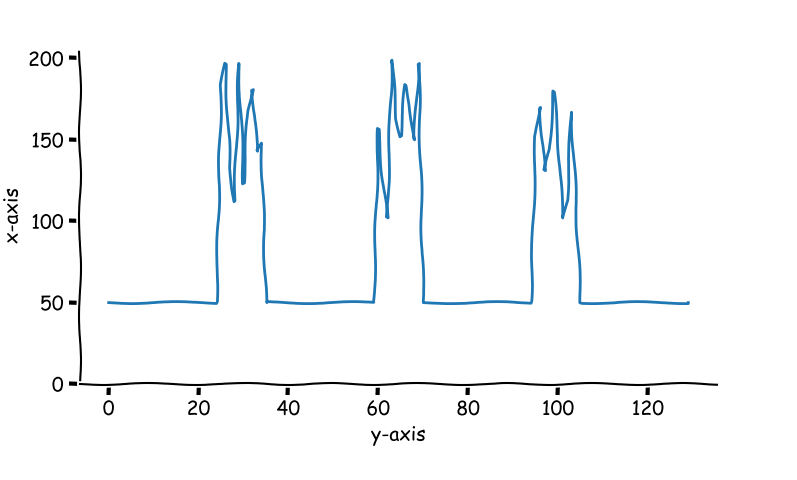
\includegraphics[width=\textwidth]{recover.png}
    \caption{Sensor recovers after some invalid reads}
    \label{fig:recover}
	\end{subfigure}
	%
	\begin{subfigure}[b]{0.3\textwidth}
    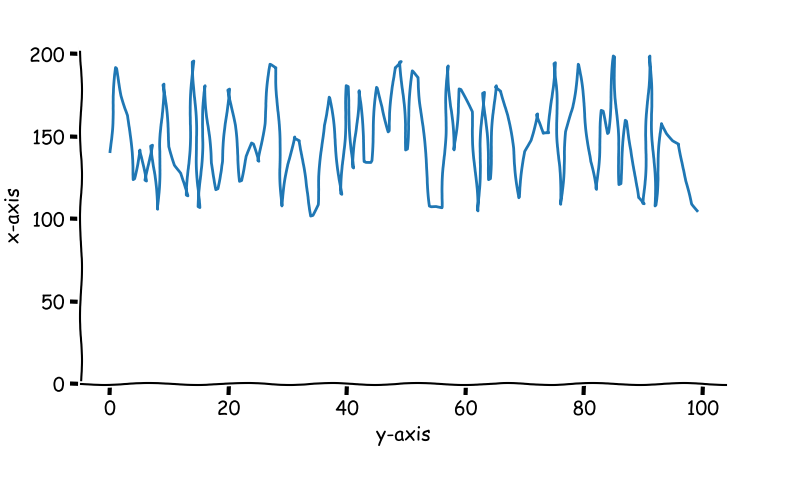
\includegraphics[width=\textwidth]{faulty_data.png}
    \caption{Sensor does not recover after invalid reads}
    \label{fig:no_recover}
	\end{subfigure}
    %
	\begin{subfigure}[b]{0.3\textwidth}
    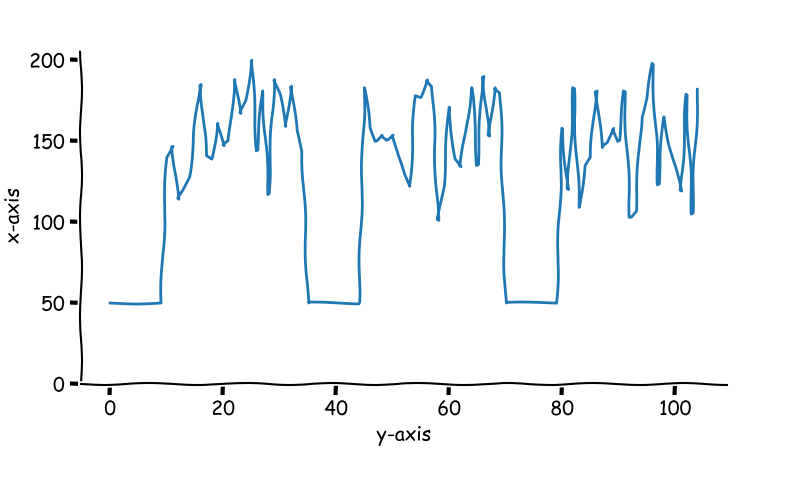
\includegraphics[width=\textwidth]{too_much_invalid.png}
    \caption{Sensor produces too much invalid data}
    \label{fig:too_much_invalid}
	\end{subfigure}
\caption{}
\end{figure}
In figure \ref{sub@fig:recover} the sensor outputs some invalid data, yet it recovers. No errors should be raised.

In figure \ref{sub@fig:no_recover} the sensor does not recover from reading invalid data, and an error should be raised.

In figure \ref{sub@fig:too_much_invalid} the sensor does recover, but still outputs enough invalid data that an error should be raised. 


\section{Sensor Disconnect}
We define a sensor disconnect as when no credible data is being produced at all. If the sensor does not recover, immediate maintenance is needed for any continued functionality. In this device we know that a sensor disconnect results in the value 0.0 being returned at every poll by the microcontroller to the sensor. While this might be a valid read in some scenarios, in a real world application we would probably never get such a stable value at exactly 0.0. Rather, it would fuzz around at maybe between 1.5 and 0.0 (for example). Disregarding this, we can also know that sensor has disconnect if the data values drop to 0.0 at a too quick pace to be a real-world measurement. 

The requirements on this device states that it should raise a disconnect error if the sensor does not recover within a given timeframe.

\begin{figure}[H]
\centering
    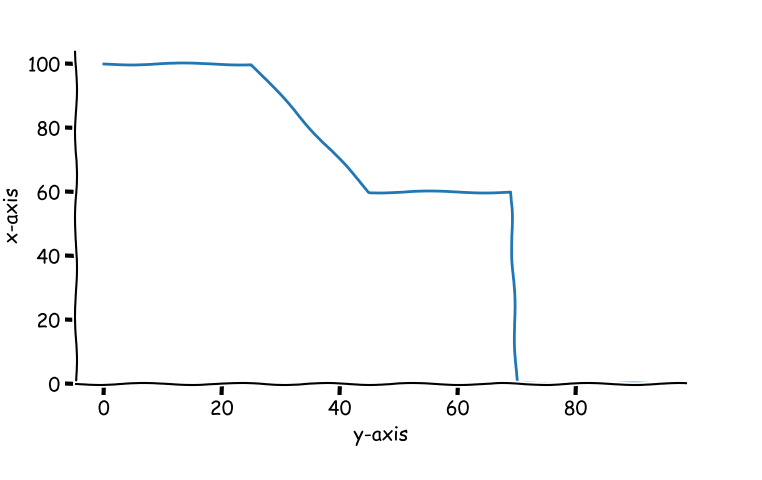
\includegraphics[width=0.3\textwidth]{disconnect.png}
    \caption{The sensor disconnects}
    \label{fig:disconnect}
\end{figure}

In figure \ref{fig:disconnect} the data values drop from 60 to 0 in the span of one data point, which would indicate a sensor disconnect.


\chapter{Design \& Implementation}
% Should be <2 pages

% **Problems**

% **Needs to contain**
% - Hardware Description on a more detailed level

% **Structure**

% - Hardware section
%     - Overview
%     - Decisions
% - Software section
%     - Overview
%     - Decisions

The work in this paper is divided up into two major areas; the hardware and the software implementations. The aim of this section is to give an overview of the implementation and the design decisions made for each area.

\section{Hardware Implementation}

% Overview
A similar paper conducted at KTH earlier this year served as the main baseline for how the hardware was to be setup.\cite{hospital} The main components are the microcontroller, the scale as well as the ADC (Analog-to-Digital Converter). Apart from this, an adequate power source is needed to provide energy to all components. 

% Decisions
\subsection{Scale}
The scale used for this paper is a Tedea Huntleigh - Model 1022. It's a small and simple model, and the specific device used in this paper had a maximum capacity of \~50 kg.\cite{load-cell-data} In figure \ref{fig:wiring} we can see the labels of the four wires needed to hook up the load cell. The \textit{Input+} and \textit{Input-} signify the voltage input and ground. \cite{load-cell-spec} \textit{Output+} and \textit{Output-} will output a positive respectively a negative charge of \~1.5 voltage . During weighing, the internal resistance in the load cell will change ever so slightly, and the two outputs will have a small difference in the millivoltage range. This difference represents the weight measurement, and can be translated to a corresponding kg/lb value. In general, the more voltage the scale is supplied with, the greater this millivoltage range can be, which (in theory) means larger accuracy when weighing. Bear in mind that no two load cells are the same, and need to be calibrated to output the correct kg/lb value. Even though no calibrations were made to the load cell during this paper, an increase in the voltage provided to the load cell did correlate to an increased stability in the values produced. 

\begin{figure}[h]
	\centering
	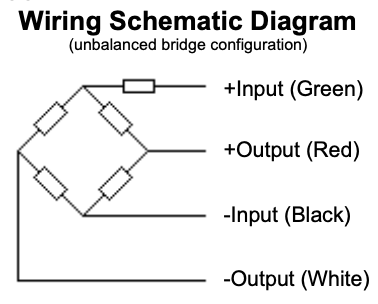
\includegraphics[width=0.3\textwidth]{load-cell-wiring.png}
	\caption{The wiring schematic for the load cell}
	\label{fig:wiring}
\end{figure}


\subsection{ADC}
To convert the millivoltage output from the load cell into a digital signal, an ADC is needed. The device used in this paper is an HX711, and apart from being a converter, it also serves as an amplifier for the load cell signal. We can see the front of the piece in figure \ref{fig:hx711}, and on the left side are the pinout where all the wires from the load cell should be connected. It's worth bearing in mind that the color coding of the wiring is not the same for all load cells, and the backside should be checked so that the connections made follow the correct wiring schematic. 

It outputs data via two of its pins, the DAT and the CLK. The CLK pin will output 0 if it's ready to send data, and 1 if it is not ready. When it is ready, the DAT pin will send  a series of 0s and 1s that can be converted from binary to a decimal value, which will then represent the output of the load scale.\cite{hx711-datasheet} Multiple code libraries have been written to handle this for the user, and the only thing left to implement is to specify which pins are being used by CLK and DAT respectively. For this paper, a library written for micropython was used.\cite{hx711-lopy}

\begin{figure}[h]
	\centering
	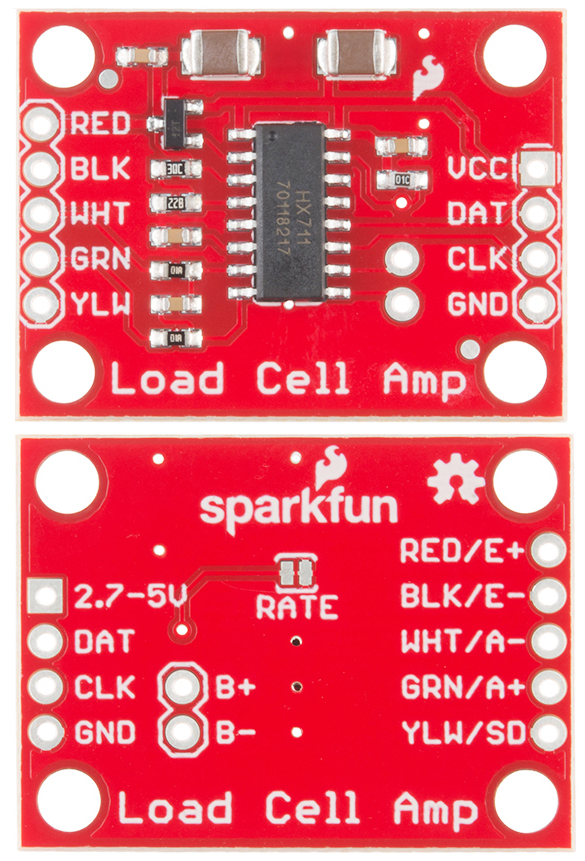
\includegraphics[width=0.3\textwidth]{hx711.png}
	\caption{The front and back of the HX711}
	\label{fig:hx711}
\end{figure}


\subsection{Microcontroller}
The microcontroller used for this paper was the FiPy development board from PyCom. It boasts a wide range of capabilities when it comes to communication protocols, NB-IoT being one of the five available.\cite{fipy-docs} With the supplied expansion board, connections via pinout is possible. It runs on micropython, which is an implementation of Python 3 optimized to run on microcontrollers.\cite{micropython}

\subsection{Power Source}
In the early stages of the project, the hardware was powered via USB cable from a computer. Since the USB was of type micro, the voltage output was at 5V. The benefit of this setup was a simple wiring schema where each component powered the next in line. The drawback was that the FiPy could only supply the ADC with 3V, which in turn affected the ADC's ability to read data from the load cell. During testing, the output rate of the raw data would be infrequent and erratic, sometimes taking several seconds to produce a single value. The values themselves did not correspond to increases and decreases in force being applied to the load cell, and would seemingly spike and crash at random. These problems were largely in part due to insufficient voltage being supplied to the ADC and load cell as later setups would reveal.

To remedy this, an approach using two different power sources was tried, where the ADC was powered by a wall outlet at a higher voltage, while the FiPy kept the USB. This resulted in electrical interference throughout the system, because of two different grounds being present in the circuit. The output rate of the data values had improved to a bit more stable rhythm than before, and the raw data values were a bit more responsive to the force applied to the load cell. 

The best setup that was tested involved an Otii battery toolbox, which is an advanced piece of hardware used to profile and emulate batteries.\cite{otii-web} With this piece of equipment, a common ground was provided to all components, as well as adequate voltage. It was capable of supplying 5V to both the FiPy and the ADC at the same time, which in turn enabled stable output of data values. When force was applied to the load cell, the data values responded accordingly with an increase or decrease in value. Due to time constraints and hardware availability, the setup could not be used for real network transmissions of the load cell data.

All data values produced by the load cell and ADC during these tests were raw values, as a calibration for kg/lb values for our intents and purposes would not bring any significant enhancements to the project.

\subsection{Wiring}
\begin{figure}[h]
	\centering
	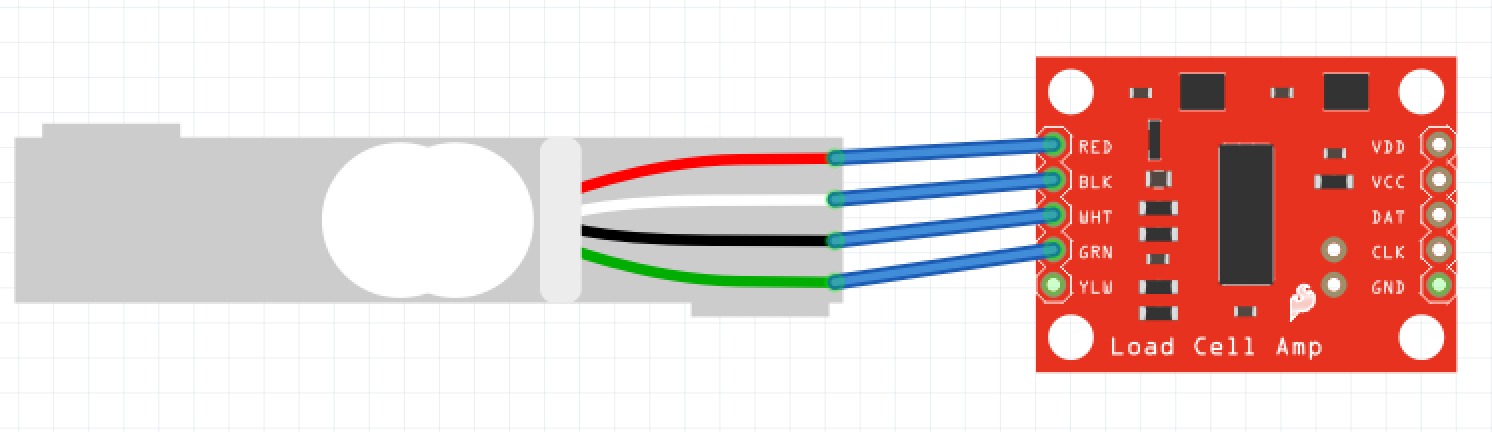
\includegraphics[width=0.6\textwidth]{load-cell_hx711.png}
	\caption{The load cell wired to the ADC}
	\label{fig:load-cell_hx711}
\end{figure}

\subsection{Failures}
During the first half of the project a faulty load cell was being used, which resulted in major delays of the hardware implementation. During the later half of the project no adequate solution to the problems with the power source could be devised in time for the practical testing of the hardware. Despite this, a short-lived setup with the Otii battery toolbox enabled a fairly functional load cell that could output tangible data values.




\section{Software Implementation}
The FiPy code runs on MicroPython, an implementation of Python 3 optimized for microcontrollers. MicroPython only executes two files on its system's root folder, the \lstinline{boot.py} and the \lstinline{main.py} files. Any remaining code must be placed in the \lstinline{lib} folder. The \lstinline{bootp.py} runs first, and is intended to contain low-level code that is meant to configure the hardware. The \lstinline{main.py} file contains the main program loop, and imports auxiliary files from the \lstinline{lib} folder.

\subsection{reader.py}
The \lstinline{reader.py} file contains the \lstinline{Reader} class, which is responsible for processing the data polled from the load cell and passing it on to being transmitted. To instantiate a functional \lstinline{reader} object, it needs to be passed a poller function as well as a transmitter function. The purpose of having these functions passed to the instance of the class instead of being hardcoded into the class is to follow the separation of concern design principle.\cite{sep-concern} The poller function should accept no argument and is expected to return the current data value produced by the load cell when called. The transmitter function in turn should accept the data value to be transmitted.

The main method of the \lstinline{reader} instance is the \lstinline{run()} method. When called, the \lstinline{run()} method performs a cycle consisting of data polling, a check for false values, adjustment of the polling rate as well as a possible transmission. 

\subsubsection{Failure Check}
The polled data value is subsequently checked for validity in the form of out-of-bounds values or extreme delta changes. A separate class called \lstinline{Fail_tracker} monitors the interval and frequency of these occurrences, and the purpose of the class is to raise an error when the error rate is deemed too high, and an administrator needs to be notified. This will result in an error message being transmitted. The internal workings of the \lstinline{Fail_tracker} will be explained in a separate section.

\subsubsection{Adjustment of polling rate}
If the value is deemed valid, it is added to a FIFO (First-in, First-out) buffer of the most recent values. The contents of the buffer are then summed into a total delta value, which is used to adjust the polling rate. If the total delta surpasses a pre-defined threshold, the polling rate is increased, whereas if it is lower it might be maintained or decreased.


\subsection{fail\_tracker.py}
The purpose of the Fail\_tracker class is to keep track of the failure occurrence and frequency. The intended usage is to instantiate an instance of the class, and call the \lstinline{strike()} method when an invalid read has occurred. This method increases an internal counter, which will then raise an exception if it passes a pre-defined threshold.

\subsubsection{GRACE\_PERIOD constant}
When invalid reads occur due to some external or internal circumstances, it might not be beneficial to count all errors within a given timeframe towards raising an exception. We are not interested in sending an alert when short periods of errors occur, instead, it is at the long-lasting periods of polling errors an exception should be raised. To account for these short bursts, we use a \lstinline{GRACE_PERIOD} constant. This constant is used for the time window after the \lstinline{strike()} method has been called, during which sequential calls  will not count towards the exception raising threshold. This time period is measured in second.

\subsubsection{COOLDOWN constant}
Since the errors 

\subsection{Data Transmissions}

\chapter{Related Work}
% TODO: Rewrite?
A similar project done at KTH in 2019 served as the main inspiration for this paper.\cite{hospital} The goal of the project was to monitor the battery levels in defibrillators via an IoT-enabled scale, and thereby optimize the battery-swapping routine. This project proved successful in it's implementation, but faced a slew of challenges that prevented it from ever being integrated into an actual user environment, due to security concerns related to the use of the hospital Wi-Fi. This shows the importance of seeing the bigger picture of where and how the device will be implemented by the end-user, and having that in mind when making technology and design trade-offs throughout the development process.

% Something related to data polling
% TODO: Cite ADP-MAC that adjusts itself on incoming traffic
One of the implementation details in this project concerned the data polling rate, which could potentially affect battery life of a sensor. The ways to regulate data polling is as varied as there are systems and devices that implement it, and apart from looking at the the energy consumption between the polling unit and the sensor, the following works look at the aspect of data polling in the context of a system, which is particularly interesting in the perspective of IoT since multiple devices will often share the same network and need to optimize the use of shared resources.

In a 2018 study by Siddiqui \etal \cite{ADP-MAC} a new protocol was developed for the MAC layer of a wireless sensor network which adjusted its polling interval depending on the rate of incoming traffic, and given certain types of traffic, was able to optimize energy and delay performance compared to another MAC protocol. 
% TODO: Cite nanonetwork polling that adjusts itself to network conditions
In a work by Yu \etal concerning electromagnetic-based wireless nano sensor networks, a polling scheme is proposed that adjusts itself according to network conditions on the IoT backhaul portion of the system, which improved bandwidth efficiency and lessened energy consumption. 

% Something related to error detection.
% TODO: Find at least two articles relating to this

\chapter{Results}
% Should be ~50% of the whole thesis
\iffalse
\begin{itemize}
	\item Don’t make the reader do all the work
	\item Have a hypothesis, test them, state result clearly
	\item Two lists are not a comparison
	\item Be the first to criticize your own work
\end{itemize}
\fi
\
\section{Hardware results}
The configuration and setup between the load cell and ADC took some time to get right, mostly due a faulty load cell being used during the first half of the project. It was also assumed that the color of the wires was standardized between load cells, so the correct wiring in figure \ref{fig:load_cell_hx711} was not implemented right away. Even though no calibrations were made to the load cell during this paper, an increase in the voltage provided to the load cell did correlate to an increased stability in the values produced. 

The second big challenge involving the hardware came from powering the project in a sufficient manner. The first power setup as seen in figure \ref{fig:wiring_comp}, was a simple and naive approach that lacked enough voltage to efficiently power the components. The benefit of this setup was a simple wiring schema where each component powered the next in line. The drawback was that the FiPy could only supply the ADC with 3V, which in turn affected the ADC's ability to read data from the load cell. During testing, the output rate of the raw data would be infrequent and erratic, sometimes taking several seconds to produce a single value. The values themselves did not correspond to increases and decreases in force being applied to the load cell, and would seemingly spike and crash at random. These problems were largely in part due to the insufficient voltage being supplied to the ADC and load cell as later setups would reveal.

% Second wiring setup
The second wiring setup was the one seen in figure \ref{fig:wiring_outlet}, and resulted in an electrical interference throughout the system, because of two different grounds being present in the circuit. This electrical interference rendered the output of the system nonsensical at time, though output rate of the data values had improved to a bit more stable rhythm than previously, and the raw data values were a bit more responsive to the force applied to the load cell..

% Third wiring setup
The third and final power setup for the project involved the Otii battery toolbox, as seen in figure \ref{fig:wiring_otii}. This setup, though a bit too advanced for a device intended to be small and simple, did produce a functioning connection between the load cell and the microcontroller. When force was applied to the load cell, the data values responded accordingly with an increase or decrease in value, and no irregularities in form of disconnects or spikes were seen in the tests. Due to time constraints and hardware availability, the setup could not be used for real network transmissions of the load cell data.

\section{Software results}

\subsection{reader.py}
The \lstinline{reader.py} file contains the \lstinline{Reader} class, which is responsible for processing the data polled from the load cell and passing it on to being transmitted. To instantiate a functional \lstinline{reader} object, it needs to be passed a poller function as well as a transmitter function. The purpose of having these functions passed to the instance of the class instead of being hardcoded into the class is to follow the separation of concern design principle.\cite{sep-concern} The type signatures for the two functions are show below. The poller function should accept no argument and is expected to return the current data value produced by the load cell when called. The transmitter function can accept a argument of any type, and should not return any value.
\begin{Code}
	def poller_function() -> value: int
	def transmitter_function(value: Any): -> None
\end{Code}


The main method of the \lstinline{reader} instance is the \lstinline{run()} method. When called, the \lstinline{run()} method performs a cycle consisting of data polling, a check for false values, adjustment of the polling rate as well as a possible transmission. 

\subsubsection{Error Check}
The polled data value is subsequently checked for validity in the form of out-of-bounds values or extreme delta changes. A separate class called \lstinline{Error_tracker} monitors the interval and frequency of these occurrences, and the purpose of the class is to raise an exception when the error rate is deemed too high, and some form of remedial action needs to be taken. The internal workings of the \lstinline{Error_tracker} will be explained in a separate section.

%TODO
\subsubsection{Disconnect Check}


\subsubsection{Adjustment of polling rate}
If the value is deemed valid, it is added to a First-in, First-out (FIFO) buffer of the most recent values. The contents of the buffer are then summed into a total delta value, which is used to adjust the polling rate. If the total delta surpasses a pre-defined threshold, the polling rate is increased, whereas if it is lower it might be maintained or decreased. The total delta value is the the delta values between two points added to the delta of the next two points, as follows:

$$\sum_{n=0}^{10} x_n - x_{n+1}$$


\subsection{error\_tracker.py}
The purpose of the Error\_tracker class is to keep track of the error occurrence and frequency. The intended usage is to instantiate an instance of the class, and call the \lstinline{error_occurred()} method when an invalid read has occurred. This method increases an internal counter, which will then raise an exception if it passes a pre-defined threshold.

\subsubsection{The Grace Period}
When invalid reads occur due to some temporary circumstance, it might not be beneficial to count all errors within a given timeframe towards raising an exception. It is not useful sending an alert when short periods of errors occur (given that very high uptime is not of importance), since this might risk producing a multitude of needless error messages. Instead, it is at the long-lasting periods of polling errors an exception should be raised. To account for short bursts of error, a constant called \lstinline{GRACE_PERIOD} is used. This constant measures the time window (in seconds) after the \lstinline{error_occurred()} method has been called, during which sequential calls  will not count toward the exception threshold.

\subsubsection{The Cooldown Period}
If errors rack up towards an exception over a longer period of time, it would lose meaning in regards to the status of the device in the short term, and would only be an indicator of long-term performance. To avoid this, the internal error counter needs to be reset or decreased periodically. To achieve this, a constant similar to the \lstinline{GRACE_PERIOD} is used, called the \lstinline{COOLDOWN} constant. This constant indicates the time window (in seconds) after the grace period, where if no calls are made to the \lstinline{error_occurred()} method, the internal error counter is decreased by one. However, if a call to the \lstinline{error_occurred()} method is made during the cooldown period, the internal error counter increases, and a new grace period starts. This way of self-regulation ensures that only a long-lasting and consistent frequency of errors raise an exception.


\subsection{Data Transmissions}
Data transmission tests were done separately from the load cell using fictional data. Pycom, the parent company behind the microcontroller used in this project also operate a cloud-based device management platform. \cite{pybytes-website} Via the pybytes platform, configuration of the network settings of the device can be managed via a firmware updater. 
In figure \ref{fig:wifi_longterm} and figure \ref{fig:wifi_raw_values} we can see data being transmitted via Wifi on a home network. The data is then displayed via graphs on the pybytes platform.

\begin{figure}[H]
\centering
	\begin{subfigure}[b]{0.4\textwidth}
    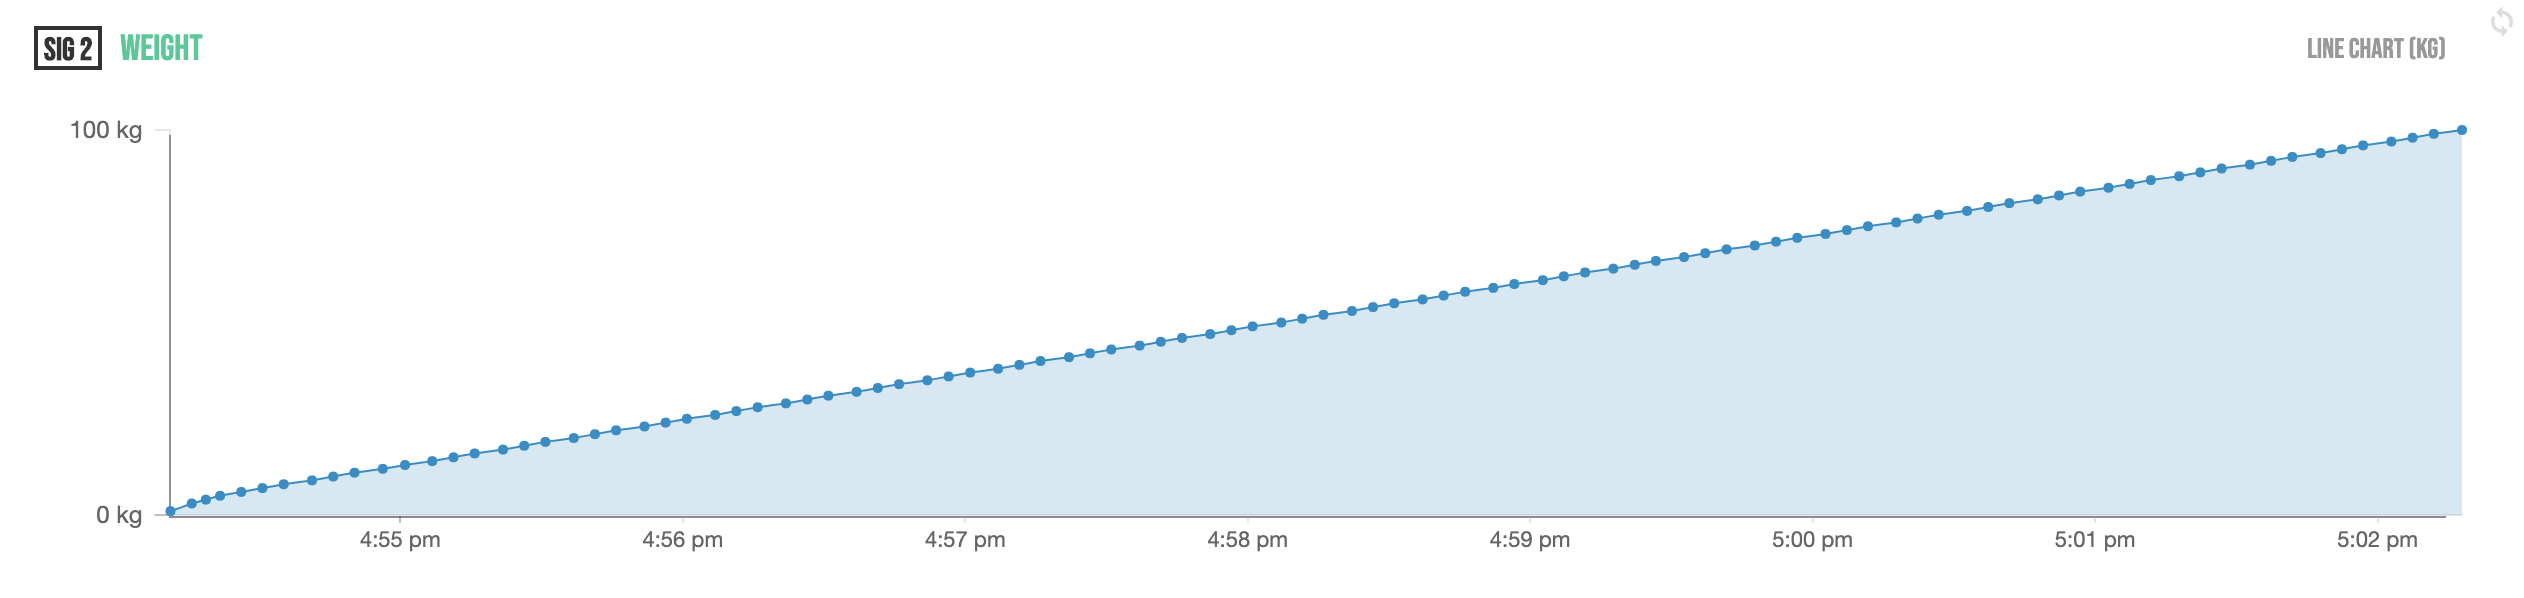
\includegraphics[width=\textwidth]{wifi_longterm.png}
    \caption{Data transmitted via Wifi}
    \label{fig:wifi_longterm}
	\end{subfigure}
	%
	\begin{subfigure}[b]{0.4\textwidth}
    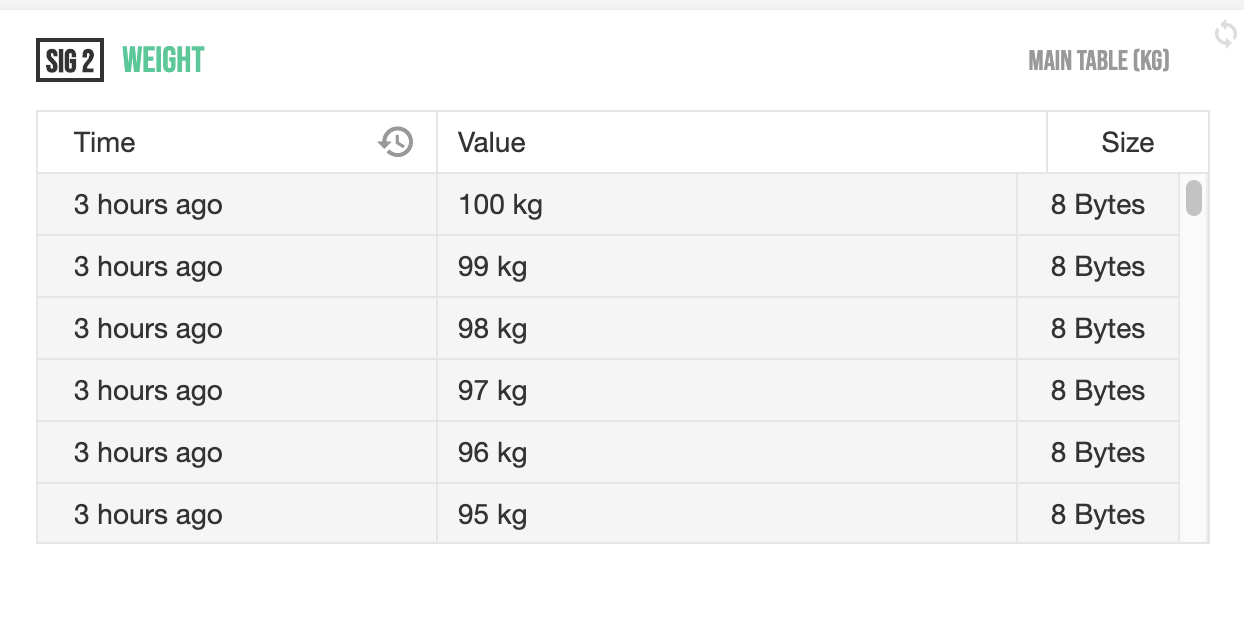
\includegraphics[width=\textwidth]{wifi_raw_values.png}
    \caption{Values transmitted via Wifi}
    \label{fig:wifi_raw_values}
	\end{subfigure}
\end{figure}

Due to time limitations in the project, no actual tests of the transmission of the data via NB-IoT were performed.
%TODO: Write more here

\section{Discussion}
%Interpretations: what do the results mean?
Despite hardships and complications when implementing the hardware, the results suggest that building and programming an NB-IoT enabled device connected to a load cell is possible with fairly simple consumer available hardware devices. It is a reasonable assumption that the hardware hindrances encountered in this paper can be bypassed with adequate planning and experience in assembling electric hardware.

%Implications: why do the results matter?
These results show a small starting point of implementing a IoT device using a load cell as its sensor. With the rise of 5G and IoT platform services there exists a real commercial interest to enable more and more actors to innovate and create products for consumers and companies alike. This project can serve as a starting point for what design and requirement considerations regarding hardware and software that need to be considered when planning and designing such a device.

\subsection{Limitations}
%Limitations: what can’t the results tell us?
%% Long term functionality
The most glaring issue with the way the hardware and software were tested during this project pertains to the time duration. When testing the connection between the load cell and microcontroller, as well as transmitting the data from the microcontroller, the tests were short compared to the intended %%TODO
%% Mass production
This project was done on a small scale, and extensive research in multiple different areas need to be conducted to even get a IoT enabled scale close to being produced for functional use, commercial or private.
%% Variance for customer
Furthermore, these results cannot account for whether the software implementation was close to emulating the desired behavior of a device from a practical standpoint, since no potential end-users were involved in the requirement specification.
%% Real life environments
Since the testing was only done indoors in a clean and controlled environment, unknown variables present in the real world could very well produce a multitude of challenges that change the way that the device works. Another interesting angle is how different locations would interact with the connection to the cellular network the NB-IoT SIM-card relies on for communication. The NB-IoT technology makes huge promises, but at the end of the day it is up to the local telecom company to fulfill the underlying conditions that make those claims possible, which would be Telia in our case.
% Duration of transmission, failure handling

% Different operators
Expanding on this, since the NB-IoT technology is fairly new in a lot of countries, there is bound to be extremely different implementation experiences from region to region depending on the network provider. In fact, NB-IoT devices could be rendered obsolete in entire regions depending on the network provider.


\chapter{Conclusions}
% Max 1 page
\iffalse
\begin{itemize}
	\item Critique
	\item Discussion
	\item Do not make the reader do all the work
\end{itemize}
\fi
%TODO: Write more here

\section{Future Work}
%% UX designer
The most focal point regarding future work to be done on this IoT scale is to involve an end-user in some shape or form early on. Ideally, a UX-designer would lead some form of market research study to more accurately specify what needs and requirements this kind of device would need to satisfy. This would be used to guide any further modifications and limitations put on the device.
%% Proper hardware assembly analysis
A more proper analyze of the needed hardware components needs to be done. Optimization in the form of hardware space, energy consumption and economical costs are essential if any more than a handful of devices are to be produced.
%% Standardized software solution
A more UX and design related question would pertain how standardized the software of the device needs to be constructed. Depending on how the use cases and market needs, can one solution fit all, or is there a way to tailor to needs in an effective way?
%% Pilot period


While the predictions and promises for the IoT industry remain hopeful and grandeur, no new devices and products will appear from thin air and propel IoT into being an integral pillar to our modern society just like that. The technology available today enables smarter products that have the potential to vastly improve our lives so long as we keep testing, trying, failing and improving. This paper was one, albeit small, test of these new technologies and many exciting projects are sure to come.

\chapter{Appendix}
\section{main.py}
\lstinputlisting[language=Python]{main.py}

\section{reader.py}
\lstinputlisting[language=Python]{lib/reader.py}

\section{test\_reader\_poll\_rate.py}
\lstinputlisting[language=Python]{lib/test_reader_poll_rate.py}

\section{error\_tracker.py}
\lstinputlisting[language=Python]{lib/error_tracker.py}

\section{test\_error\_tracker.py}
\lstinputlisting[language=Python]{lib/test_error_tracker.py}

\section{unittest.py}
\lstinputlisting[language=Python]{lib/unittest.py}

\bibliographystyle{plainnat}
\bibliography{main}

\end{document}

%%% Local Variables: ***
%%% mode: latex ***
%%% TeX-master: "main.tex"  ***
%%% ispell-local-dictionary: "British"  ***
%%% End: ***